\cotefile{157-2}
\scanpage{211}\mspage{156}

% MS 1–2
b) Si $X$ et $Y$ sont lisses sur $S$, cet élément \unsure{s'interprète|s'interprête} comme

% MS 3
\[
 \mathrm{hot}_{S,\unsure{W|w}}(X)\times_S\mathrm{hot}_{S,W}(Y).
\]

% MS upper left beside b–c
% slanted
\margin{Mais aussi si l'\uline{un} des deux éléments est dans $\uline{\mathrm{Fibhot}}\,S$ (et \unsure{moyennant} l'axiome L6 bis sur $W$)}

% MS 4–8
c) Si l'un des deux $X,Y$ \deleted{\unsure{sont}}\unsure{est} lisse sur $S$, sans rien supposer sur \deleted{\unsure{l'}}l'autre, on a une interprétation en termes de $\mathrm{mult}_X$ (si $Y$ lisse), ou $\mathrm{mult}_Y$ (si $X$ lisse), \unsure{notamment}

% MS 9–12
\[
\begin{aligned}
 \mathrm{hot}_{S,W}(X\times_S Y)&\simeq\mathrm{multhot}_X(\mathrm{hot}_{S,W}(Y))\\
 &\hspace{3em}\text{si $Y$ lisse sur $S$}\\
 \deleted{\mathrm{hot}_{S,W}(}&\simeq\mathrm{multhot}_Y(\mathrm{hot}_{S,W}(X))\\
 &\hspace{3em}\text{si $X$ lisse sur $S$.}
\end{aligned}
\]

% MS 13–15
\uline{Corollaire 2} Soit $f:S'\longrightarrow S$ une flèche de $\mathrm{Cat}$, d'où $f_!,f^*$ \deleted{\unsure{;}} entre $\mathrm{HOT}_W(S')$ et $\mathrm{HOT}_W(S)$. On a la relation

% MS 16
\[
 f_!f^*(\unsure{\xi|\zeta})\simeq\mathrm{multhot}_{S'}(\xi),
\]

% MS 17
donc si $S'$ est lisse sur $S$

% MS 18
\[
 f_!f^{\unsure{\circ|*}}(\unsure{y|\xi})\simeq\mathrm{hot}_{S,W}(S')\times_S\xi.
\]

% MS 19–25
Nous sommes maintenant en mesure de vérifier les axiomes Dér \unsure{4'b|4''b} ; Der $5'$ relatifs aux \unsure{images} \unsure{directes}, \inserted{(I \unsure{\S\,p.|pp.}\ 67,68)} et de plus Der 3 b (I p.~111). L'axiome Der $4'$ n'est autre que l'existence des adjoints à gauche \inserted{\unsure{$f_!$}} des $f^*$. L'axiome Dér $5'$ \deleted{\unsure{précise}}\inserted{permet} le ``calcul'' des fibres \deleted{de}\inserted{d'un objet} $f_!(\xi)$. Il dit qu'une certaine

% archive sheet number: 210
\scanpage{212}\mspage{157}

% MS 1–2
flèche de chgt de base, relative au \deleted{\unsure{foncteur|le foncteur} $f_!$,}\inserted{diagramme} commutatif de $\mathrm{Cat}$

% MS 3–5 upper square
\diagram{\begin{tikzcd}[ampersand replacement=\&]
 S' \arrow[d,"f"'] \& {}_{s\backslash}S' \arrow[l,"q"'] \arrow[d,"f'"] \\
 S \& e\simeq\{s\} \arrow[l,"p"'] \& (s\in\mathrm{Ob}\,S)
\end{tikzcd}}

% MS 6
savoir

% MS 7
\[
 p^*(f_!(\unsure{\xi|\zeta}'))\longrightarrow f'_!(q^*(\xi')
\]

% MS 8
est un isomorphisme (pour $\xi'\in\mathbb D(S')$).

% MS 9
Soit donc

% MS 10
\[
 \xi'\in\mathrm{Ob}\,\mathrm{HOT}_{\unsure{W|w}}(S'),\qquad
 \xi'=\mathrm{hot}_{S',W}(X')
\]

% MS 11
avec $X'$ dans $\mathrm{Cat}_{/S'}$. \unsure{Comme} \deleted{\unsure{le}}

% MS 12
\[
 f_!(\xi')=\mathrm{hot}_{S,W}(X'),
\]

% MS 13–19
et que $X'$ n'a \deleted{\unsure{t}} aucune raison d'être lisse sur $S$ (si on ne suppose pas $S'$ \inserted{lui-même} lisse sur $S$, auquel cas il pourrait être utile de \deleted{se \unsure{restreindre}} prendre $X'$ \deleted{\unsure{lui-même}} lisse sur $S'$, donc aussi sur $S$), pour calculer $p^*(f_!(\unsure{y|\xi}'))$, il n'est pas question de prendre la fibre $X'_s$, mais il faut prendre $ {}_{s\backslash}X'=\unsure{\Phi|\varPhi}_S(X')_{\unsure{-s|s}}$ :

% MS 20
\[
 p^*(f_!(\xi'))\simeq\mathrm{hot}_W({}_{s\backslash}X').
\]

% MS 21–24 lower left square pair
\diagram{\begin{tikzcd}[ampersand replacement=\&]
 X' \arrow[d] \& {}_{s\backslash}X' \arrow[l] \arrow[d] \\
 S' \arrow[d] \& {}_{s\backslash}S' \arrow[l,"q"'] \arrow[d] \\
 S \& {}_{s\backslash}S \arrow[l]
\end{tikzcd}}

% MS 21–27 beside and below squares
Considérons le diagramme de chgt. de base par $ {}_{s\backslash}S\longrightarrow S$ ci-contre, à carrés cartésiens. On voit d'abord que $q^*(\xi')$ n'est autre que \deleted{$\mathrm{hot}_{{}_{s\backslash}S',W}({}_{s\backslash}\unsure{S'|X'})$} la classe dans $\mathrm{HOT}_W({}_{s\backslash}S')$ de l'image inverse de $X'$ par le chgt de base $ {}_{s\backslash}S'\longrightarrow S'$. Pour l'assurer, il suffirait de prendre $X'$ lisse sur $S'$. \unsure{(ce qui|(celui qui}

% archive sheet number: 211
\scanpage{213}\mspage{158}

% MS 1–5
est licite) -- \deleted{\unsure{alors}} la description de l'image inv. est OK pour \uline{\unsure{tt}} chgt de base. Mais on a vu que dans le cas d'un \unsure{voisin|voisinage} local comme $ {}_{s\backslash}S'\longrightarrow S'$, il n'y a pas même besoin de cet artifice -- la formule est OK sans restriction de lissité.

% MS 6
\deleted{\unsure{Comme le}}\inserted{Ainsi}

% MS 7
\[
 q^*(\unsure{\xi|\zeta}')\simeq\mathrm{hot}_{{}_{s\backslash}S',\unsure{W|w}}({}_{s\backslash}X'),
\]

% MS 8
d'où

% MS 9
\[
 f'_!(q^*(\xi'))\simeq\mathrm{hot}_{\unsure{e|S},W}({}_{s\backslash}X')=\mathrm{hot}_W({}_{s\backslash}X').
\]

% MS 10
Donc on a bien trouvé

% MS 11
\[
 p^*f_!\simeq f'_{\unsure{!|!*}}q^*.
\]

% MS 12–15
On peut maintenant prouver aussi Der 3 b. On a vu qu' \deleted{\unsure{une}} fois qu'on dispose des adjoints à gauche $f_!$ des $f^*$, cet axiome s'énonce sous \uline{forme homologique} ainsi :

% MS 16
Si

% MS 17
\[
 f:S'\longrightarrow S
\]

% MS 18–19
est dans $W$, il faut prouver que pour tout

% MS 19
\[
 \xi\in\mathrm{HOT}_W(e)\overset{\mathrm{def}}{=}\mathrm{Hot}_W
\]

% MS 20
la flèche correspondante

% MS 21
\[
 \unsure{f'|p'}_!\,p'^*(\xi)\longrightarrow p_!p^*(\xi)\tag*{$(*)$}
\]

% MS 22–25
est iso dans $\mathrm{Hot}_W$, où $p:S\longrightarrow e$, $p':S'\longrightarrow e$ sont les flèches structurales. Or comme tout objet de $\mathrm{Cat}$ est lisse sur $e$, le cor.~2. précédent permet d'identifier cette flèche \unsure{bis|bas|les} :

% MS 26
\[
 \unsure{s|S}'\times_S\xi\longrightarrow s\times_S\xi
\]

% archive sheet number: 212
\scanpage{214}\mspage{159}

% MS 1
déduite de

% MS 2–3
\diagram{\begin{tikzcd}[ampersand replacement=\&,column sep=small,row sep=0.2em]
 \mathrm{hot}_{\unsure{W|w}}(f): \& \unsure{s|S}' \arrow[r,"{\deleted{\unsure{\mathrm{hot}(f)}}}"] \& s\\
 \& \overset{\mathrm{def}}{\shortparallel} \& \overset{\mathrm{def}}{\shortparallel}\\
 \& \mathrm{hot}_W(S') \& \mathrm{hot}_W(S)
\end{tikzcd}}

% MS 4–5
Comme celle-ci est iso \inserted{par hypothèse}, on gagne.

% MS 6
Donc on a prouvé

% MS vertical rule beside proposition
\margin{\figure{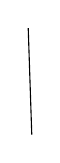
\begin{tikzpicture}[x=1mm,y=1mm]\draw (0,0)--(-0.45,13.5);\end{tikzpicture}}}

% MS 7–9
\uline{\deleted{\unsure{Théorème}}\unsure{Proposition} 3} Le prédérivateur $\mathrm{HOT}$ satisfait aux axiomes Der 1, Der 2 \inserted{(pour mémoire)} et Der $3\,b^{*}$, Der $4'$ \deleted{\unsure{b}}, Der $5'$.

% MS upper right, arrow from Der 2
% slanted
\margin{\uline{pas prouvé} \deleted{\illegible{5}} le ``résultat'' auquel je suis \unsure{``parvenu''} \unsure{est} \unsure{cf. n\textsuperscript{o} 5} p.~165}

% MS right below the proposition
\margin{cf complément prop.~\uline{5} p.~\unsure{167|164}}

% MS left beside Der 3 b
% slanted
\margin{et \unsure{$=$|$\Longleftarrow$} la variante la plus forte Der $3\,b'_2$ de Der 3, cf \unsure{aussi} page suivante.}

% MS left below preceding note
% slanted
\margin{\uline{NB} Pour D $3\,b'_2$, on a utilisé l'axiome L6 ``$W$ est \unsure{dit|clos} \unsure{cf} \unsure{multiplicatif}''. \deleted{et On} voit que $\times_*$ \unsure{la validité} de Der $3\,b'_2$ implique L6 \unsure{bis}, et même la forme plus forte L6 bis, dans cette forme si on exige seulement \unsure{donc} $3\,b''_1$ \unsure{pour} $f_0^*$ pl. fid.}

% MS 10–13
On vient de prouver aussi les variantes \unsure{inférieures} de Der 3, la forme la plus forte de celles-ci (Der $3\,b'_2$) : si $f\in W$, alors $f^*$ induit une \uline{équivalence} de catégories

% MS 14
\[
 f_0^*:\mathrm{HOT}_W^{\mathrm{lc}}(S)\longrightarrow\mathrm{HOT}_W^{\mathrm{lc}}(S').
\]

% MS 15–23
La pleine fidélité du foncteur $f_0^*$ doit résulter de \deleted{Der 3 b} la variante naturelle Der $3\,b''_{\mathrm{coh}}$ de Der 3 b, une fois qu'on aura développé le formalisme des \deleted{\unsure{foncteurs}} Homs internes dans les $\mathrm{HOT}_{\deleted{\unsure{V}}W}(\deleted{\unsure{s}}S)$. Mais \deleted{\unsure{pour}} donner un sens à Der $3\,b''_{\mathrm{coh}}$, on a besoin des foncteurs \uline{cohomologiques}, i.e. de $p_*$ et $p'_*$ \unsure{(au} lieu de $p_!$, $p'_!)$ pour $\mathrm{HOT}$, donc c'est encore prématuré pour l'instant. La construction des $f_*$ et celle des Homs internes \deleted{\unsure{est}}\inserted{\unsure{fera|sera}} d'ailleurs sûrement $\pm$ \unsure{conjointement}.

% archive sheet number: 213
\scanpage{215}\mspage{159}
% archive sheet number: 214

% MS 1–8
Mais je m'aperçois à l'instant qu'on \unsure{trouve|tourne} quasiment ``à l'œil'' le fait que $f_0^*$ soit bien une \uline{équivalence} de \unsure{catégorie|catégories}, et que $f_!^0$ soit l'équivalence quasi-inverse, en utilisant l'adjonction des foncteurs $f_!^0,f_0^*$, et se \unsure{rappellant|rappelant} que pour prouver que ce sont des équivalences quasi-inv. l'une de l'autre, il \deleted{suffit}\inserted{revient au même} de montrer que les morphismes d'adjonction

% MS 9–10
\[
\begin{aligned}
 \mathrm{id}&\xrightarrow{\alpha_0} f_0^* f_!^0\\
 \mathrm{id}&\xleftarrow{\beta_0} f_!^0 f_0^*
\end{aligned}
\]

% MS 11
sont \uline{iso}.

% MS 11–14 crossed block
\deleted{J'admets que ces flèches sont données par le $=$ \unsure{procédé|précédent} que dans le cas de $f_!,f^*$, 1) $\alpha_0$ est iso. Je prends $\unsure{\xi|\zeta}'\in\mathrm{Ob}\,\mathrm{HOT}^{\mathrm{lc}}_{\unsure{W|w}}(S')$, il est défini par $X'\in\mathrm{Ob}\,\deleted{\mathrm{Cat}_{/S'}}\,\unsure{\mathscr P|\mathscr S}_{S'}$ comme}

% MS 15–16 crossed display
\[
\deleted{\begin{aligned}
 \xi'&=\mathrm{hot}_{S',W}^{\mathrm{lc}}(X'),\ \text{d'où}\quad
 f_!^0(\xi')=\mathrm{hot}_{S,W}^{\mathrm{lc}}(X'),\quad
 f_0^*f_!^0(\xi')=\mathrm{hot}_{S',W}(C_S(X')\times_S S'),\\
 &\hspace{8em}=\mathrm{hot}_{S,W}(C(\unsure{X'|X}))
\end{aligned}}
\]

% MS 17–19
Je vais essayer de décrire ces flèches d'adjonction dans le cas général (sans supposer $f\in W$), puis de montrer qu'elles sont dans $W$ si $f$ l'est.

% MS 20
$\xi=\mathrm{hot}_{S,W}^{\mathrm{l.c.}}(X)$ dans $\mathrm{HOT}_W(S)$ \unsure{OTS|OOT|OOI} $X\in\mathrm{Ob}\,\uline{\mathrm{Parf}}\,S$.

% MS 21
\deleted{Comme} $X$ lisse sur $S$, on a

% MS 22–23
\[
\begin{aligned}
 f_0^*(\xi)&=\mathrm{hot}_{S',W}^{\mathrm{lc}}(X\times_S S'),\quad
 f_!^0 f_0^*(\xi)=\mathrm{hot}_{S,W}^{\mathrm{lc}}(X\times_S S')\\
 &\hspace{12em}\deleted{{}=\mathrm{hot}_{S,W}^{\mathrm{lc}}(C_S(X\times_S S'))}
\end{aligned}
\]

% MS 24–25
Donc \deleted{\unsure{$f_0^*$})} $\beta_{0\,\xi}:f_!^0f_0^*(\xi)\longrightarrow\xi$ flèche

% MS 26
\[
 X\times_S S'\longrightarrow X\qquad\text{dans }(\mathrm{Cat}_{/S})(W_S)^{-1}
\]

% MS lower left, alongside 24–27
% slanted
\margin{\uline{NB} On voit que l'axiome L6 est $\pm$ \uline{nécessaire} pour que la \unsure{validité} du \unsure{calcul} $f_0^*$, $f_!^0$ \unsure{soit|ait une} \unsure{valable|valeur}}

% MS 27–28
Je présume que c'est \unsure{$\mathrm{pr}_1$|$\mathrm{pr}\,1$}. Est-ce dans $W$ si $f:S'\longrightarrow S$ l'est ? Oui, car $X$ est parfait
\scanpage{216}\mspage{161}

% MS 1–2
sur $S$), sous réserve que $W$ satisfait l'axiome L \unsure{5|6} (cf page 43).

% MS 3
2) Soit

% MS 4
\[
 \unsure{\xi|\zeta}'\deleted{\unsure{\in}}=\mathrm{hot}_{S',\unsure{W|w}}^{\mathrm{lc}}(X')\quad\text{dans }\mathrm{HOT}_W(S'),
\]

% MS 5
on a $f_!^0(\xi')=\mathrm{hot}_{S,W}^{\mathrm{lc}}(X')$,

% MS 6–9
mais pour expliciter $f_0^*$ \deleted{\unsure{$\xi$}} de cet élément, comme $X'$ n'a aucune raison d'être \deleted{\unsure{fibré} fibré} un \unsure{HA|H$\Lambda$}-fibré sur $S$ (auquel cas il suffirait de prendre $f^*(X')\overset{\mathrm{def}}=X'\times_S S'$), il faut d'abord prendre $C_S(X')$, puis appliquer $f^*$ :

% MS 10
\[
 f_0^*f_!^0(X')=\deleted{\unsure{C_S(X')}}\mathrm{hot}_{S',W}^{\mathrm{lc}}(C_S(X')\times_S S')
\]

% MS 11
Il faut donc définir

% MS 12
\[
 X'\xrightarrow{\beta_{0\,X'}} C_S(X')\times_S S'
 \qquad\text{dans }(\mathrm{Cat}_{/S'})W_{S'}^{-1}.
\]

% MS 13–15
Or on trouve une flèche canonique dans $\mathrm{Cat}_{/S'}$, déduite du $S$-morphisme $i_{X'}:X'\unsure{\text{---}|\longrightarrow} C_S(X')$ i.e. du carré comm. en traits pleins

% MS 16–18
\diagram{\begin{tikzcd}[ampersand replacement=\&,column sep=small,row sep=small]
 X'\arrow[rr,no head,"i_{X'}"]\arrow[dd,"p_{X'}"']\arrow[dr,dashed,"{\beta_{0\,X'}}"'] \& \& C_S(X')\arrow[dd]\\
 \& C_S(X')\times_S S'\arrow[ur,dashed,"{\mathrm{pr}_1}"']\arrow[dl,dashed]\arrow[d,phantom,"{\text{\unsure{comm.}}}"] \&\\
 S'\arrow[rr,"f"] \& \& S
\end{tikzcd}}

% MS punctuation at right of square
,

% MS 19–21
comme l'unique flèche pointillée $\beta_{0\,X'}$ qui soit un $S'$-morphisme (triangle gauche comm.) et qui rende commutatif le triangle supérieur.

% MS 22–25
Si $f\in W$, alors $\mathrm{pr}_1$, déduit de $f$ par chgt. de base $C_S(X')\longrightarrow S$ qui est parfait, est dans $W$ par L 5, on sait qu'il en est de $=$ de $i_{X'}$, donc aussi de $\beta_{0\,X'}$, on gagne !

% archive sheet number: 215
\scanpage{217}\mspage{162}

% MS 1–3
Pour terminer les propriétés générales des foncteurs $f_!$ pour $\mathrm{HOT}_{\unsure{W|w}}$, je voudrais donner les énoncés \unsure{raisonnables|vraisemblables} de chgt. de base.

% MS 4
Ce serait un

% MS 5
\uline{Théorème}\unsure{$'$} \deleted{\unsure{(?)}} 4 \deleted{\unsure{(provisoire)}}. Soit

% MS 6–8
\diagram{\begin{tikzcd}[ampersand replacement=\&]
 X\arrow[d,"f"'] \& X'\arrow[l,"q"']\arrow[d,"f'"]\\
 S \& S'\arrow[l,"p"']
\end{tikzcd}}

% MS 8–10
un diagramme cartésien dans $\mathrm{Cat}$, considérons la flèche de chang\textsuperscript{mt} de base (dans $\uline{\mathrm{Hom}}(\mathrm{HOT}_W(X),\mathrm{HOT}_W(S'))$) :

% MS 11
\[
 p^*f_!\unsure{\longleftarrow|\longleftrightarrow}f'_!q^*.
\]

% MS 12
C'est un iso dans chacun des deux cas suivants :

% MS 13
a) $f$ est \deleted{propre} lisse

% MS 14
b) $p$ est propre.

% MS left of cases
% slanted
\margin{\deleted{Le cas a) \unsure{sera|est} établi, le cas b) reste à prouver.}}

% MS right of cases
\margin{\deleted{Il \unsure{résulte|résulterait} de Der 2 (\unsure{critère de localisation}) pour $\mathrm{HOT}$, \unsure{dans|donc} $\mathrm{HOT}_W(S')$, qu'il est \unsure{par contre prouvé}}}

% MS 15–16
\uline{\unsure{Dét.|Dém.}} Cas a). On teste avec $\unsure{\xi|\zeta}$ dans $\mathrm{HOT}_W(X)$, \unsure{objet} $\xi$ de la forme

% MS 17
\[
 \xi=\mathrm{hot}_{\unsure{X|S},W}(Z)\qquad\text{avec }Z\in\mathrm{Ob}\,\uline{\mathrm{Liss}}\,X,
\]

% MS 18–19
Notons que $Z$ est alors aussi lisse sur $S$, puisque $f$ est lisse.

% MS 20–21
\[
\begin{aligned}
 f_!(\xi)&=\mathrm{hot}_{S,W}(Z),\quad p^*f_!(\xi)=\mathrm{hot}_{S',W}(\underbrace{Z\times_S S'}_{\shortparallel\ Z',\,\text{cf diagr.}}).\\
 q^*(\xi)&=\mathrm{hot}_{X',W}(Z'),\quad f'_!q^*(\xi)=\mathrm{hot}_{S',W}(Z'),
\end{aligned}
\]

% MS lower left accompanying diagram
\diagram{\begin{tikzcd}[ampersand replacement=\&]
 Z\arrow[d] \& Z'\arrow[l]\arrow[d]\\
 X\arrow[d,"f"'] \& X'\arrow[l,"q"]\arrow[d,"f'"]\\
 S \& S'\arrow[l,"p"]
\end{tikzcd}}

% MS 22
OK !

% MS 23
\uline{Cas b)} Il faut admettre que

% archive sheet number: 216
\scanpage{218}\mspage{163}

% MS 1
le foncteur chgt de base par $p$ : \deleted{transforme}

% MS 2
\[
 Z\longmapsto Z\times_S S':\mathrm{Cat}_{/S}\unsure{\mathord{-}|\longrightarrow}\mathrm{Cat}_{/S'}
\]

% MS 3–6
est compatible avec les localiseurs $\unsure{W|w}_S^d,W_{S'}^d$ (cf plus bas) -- c'est ça, finalement, la propriété pertinente pour $p$.$^*$ Il en résulterait que

% MS left of 4–8
% slanted
\margin{Ça doit être \uline{équivalent} à $p$ propre. Comme je \unsure{vais} \unsure{voir} le cor.~2 page 166}

% MS 7
\[
 p^*:\mathrm{HOT}_W(S)\unsure{\mathord{-}|\longrightarrow}\mathrm{HOT}_W(S')
\]

% MS 8–10
se calcule, pour un élément dans $\mathrm{HOT}_W(S)$ donné par un $Z$ \uline{quelconque} dans $\mathrm{Cat}_{/S}$ (pas néc. lisse sur $S$), par

% MS 11
\[
 p^*(\mathrm{hot}_{S,W}(Z))=\mathrm{hot}_{S',W}(Z\times_S S').
\]

% MS 12–16
Partant alors \inserted{comme dans a),} d'un élément $\unsure{\xi|\zeta}$ de $\mathrm{HOT}_{\deleted{\unsure{X}},W}(X)$ donné par un $Z$ de $\mathrm{Cat}_{/X}$ (inutile cette fois de supposer $Z$ lisse), le calcul immédiat précédent établit encore la formule de commutation.

% MS 17–23
Mais \unsure{j'ai|il} \unsure{ne|me} semble pas que la propriété de compatibilité de $X\longmapsto X\times_S S'$ avec la \deleted{\unsure{$W$-}}\unsure{équivalence} colocale sur $S$ et sur $S'$, résulte de façon $\pm$ évidente de la condition pour $p:S'\longrightarrow S$ soit propre. J'ai envie de la déduire de \unsure{théorèmes} sur le formalisme des dérivateurs, à savoir des th. de chgt. de \unsure{bases} des $f_!^{\mathbb D}$ par un morphisme $\mathbb D$-propre.

% MS bottom left beside final paragraph
% slanted
\margin{Mais si, cf \unsure{dém.|idem|dessin.} page 168. \unsure{tous|seult} les développements des quatre à \unsure{cinq} pages qui suivent \unsure{ont été faits} \unsure{sans tenir compte} de \unsure{cette chose|ces choses}}

% archive sheet number: 217
\scanpage{219}\mspage{164}

% MS 1–4
Sous forme duale d'un th. de chgt. de base pour $f_*^{\mathbb D}$, par chgt de base $\mathbb D$-lisse, c'est fait dans I p.~\unsure{56|66} ; 58, et on doit pouvoir l'appliquer ici.

% MS 4–11
\deleted{Nous} Notons que dans la dém. du th. \unsure{loc. cit.}, on n'utilise que l'existence des $f_*^{\mathbb D}$ \inserted{\unsure{L 4 i.e.|L 4 inv.}}, à l'exclusion des $f_!^{\mathbb D}$ \inserted{(L $4'$)}, plus L 5 bien sûr, donc la forme duale ne \deleted{\unsure{doit pas}} fait \unsure{appel} à l'existence des $f_*^{\mathbb D}$, seulement des $f_!^{\mathbb D}$, On a donc une bonne chance de pouvoir l'appliquer à $\mathrm{HOT}_{\unsure{W|w}}$ (où je n'ai pas encore établi l'existence des $f_*^{\mathrm{HOT}}$).

% MS 12
Notons d'abord

% MS left edge of proposition
\margin{\figure{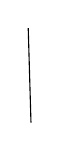
\begin{tikzpicture}[x=1mm,y=1mm]\draw (0,0)--(-0.35,12);\end{tikzpicture}}}

% MS 13–17
\uline{Proposition} 5. Soit $f:S'\longrightarrow S$ une flèche dans $\mathrm{Cat}$. Alors $f$ est une $\mathrm{HOT}_W$-équivalence \uuline{sss} \deleted{c'est une \unsure{Hot} $f$ est dans $W$.} \inserted{$\mathrm{hot}_W(f)$ est iso.} Si $W$ est fortement saturé, cela signifie donc que \deleted{\unsure{ssi}} $f\in W$ (et \unsure{$=$} \unsure{en fait contenu} \inserted{$f\in W\Rightarrow$ une $\mathrm{HOT}_W$-équivalence} dans le \unsure{$+$} démonstration de Der 3 b \deleted{\unsure{tantôt}}.

% MS left beside proposition
% slanted
\margin{devrait remonter avec le th.~3 p.~159}

% MS 17–19
Je rappelle que $f$ est une $\mathrm{HOT}$-équiv., par définition, sss pour \deleted{\unsure{les couples}} $a,b\in\mathrm{Hot}_W$ ($=\mathrm{HOT}_W(e)$),

% MS 20
\[
 \mathrm{Hom}_{\mathrm{HOT}_W(S)}(a_S,b_S)\unsure{\mathord{-}|\longrightarrow}
 \mathrm{Hom}_{\mathrm{HOT}_W(S')}(a_{S'},b_{S'})
\]

% MS 21–24
est iso, où $a_S$ \unsure{etc|est} désigne $p_S^*(a)$ etc ($p_S:S\longrightarrow e$). La formule d'adjonction de $p_{S!},p_S^*$ et de $p_{S'!},p_{S'}^*$ permettent d'interpréter la flèche \unsure{ci$_S$|can.} comme

% MS 25
\[
 \mathrm{Hom}_{\mathrm{Hot}_W}\unsure{\in}(p_{S!}(a_S),b)\longrightarrow
 \mathrm{Hom}_{\mathrm{Hot}_W}(p_{S'!}(a_{S'}),b),
\]

% archive sheet number: 218
\scanpage{220}\mspage{165}

% MS 1–2
déduite par ``transposition'' ($\mathrm{Hom}(-,b)$) de la flèche

% MS 3
\[
 p_{S'!}(a_{S'})\longrightarrow p_{S!}(a_S)
\]

% MS 4–6
induite par $f$ -- donc il faut prouver que celle-ci est un iso (c'est la forme que nous avions utilisée tantôt). Or cette flèche s'identifie à

% MS 7
\[
 \unsure{s|S}'\times a\longrightarrow s\times a
\]

% MS 8
induite par

% MS 9–10
\diagram{\begin{tikzcd}[ampersand replacement=\&,column sep=small,row sep=0.2em]
 \mathrm{hot}_{\unsure{W|w}}(f): \& s'\arrow[r,no head] \& s\\
 \& \shortparallel \& \shortparallel\\
 \& \mathrm{hot}_W(S') \& \mathrm{hot}_W(S)
\end{tikzcd}}

% MS 10
,

% MS 11–14
et dire que c'est iso quel que soit $a$, dans $\mathrm{Hot}_W$, revient à dire que $s'\longrightarrow s$ l'est (puisque la multiplication dans $\mathrm{Hot}_W$ a un élément unité \ldots)

% MS 15–22
Maintenant je me rappelle que pour avoir l'axiome Der 2 des dérivateurs, je devais également supposer $W$ \uline{fortement} \unsure{saturée|saturé} (i.e. égale au localiseur défini par le foncteur canonique $\mathrm{Cat}\longrightarrow(\mathrm{Cat})W^{-1}\overset{\mathrm{def}}{=}\mathrm{Hot}_W$). (\unsure{C'est} ce que je supposais d'emblée, en partant d'un $(M,W)$ \inserted{général}, pour définir un prédérivateur, pour avoir l'axiome Der 2.)

% MS 23–25
En appliquant le dual du th. de I, p.~\unsure{56|50}, on trouve donc le th. de chgt. de base pour $f_!$, pour chgt de base $p:S'\longrightarrow S$ \inserted{$W$-}\uline{propre}.

% archive sheet number: 219
\scanpage{221}\mspage{166}

% MS left margin beside lines 1–4
\margin{\figure{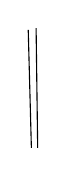
\begin{tikzpicture}[x=1mm,y=1mm]\draw (0,0)--(-0.4,15);\draw (0.8,0)--(0.6,15.2);\end{tikzpicture}}}

% MS 1–5
Mais la démonstration utilise sûrement Der 2, \deleted{\unsure{que je}} (critère d'iso par fibres, dans $\mathrm{HOT}_{\unsure{W|w}}(S)$), que je n'ai pas prouvé encore. Elle est incomplète pour le moment. Mais je peux noter dès maintenant le

% MS 6–12
\uline{Corollaire 1} (du théorème 4. p.~162) Si la flèche $S'\xrightarrow{p}S$ dans $\mathrm{Cat}$ donne lieu (pour \deleted{\unsure{$X$ fixé dans}}\inserted{tout} $f:X\longrightarrow S$ \deleted{fixé} dans $\mathrm{Cat}_{/S}$) à la formule de changement de base pour $f_!:\mathrm{HOT}_W(X)\unsure{\mathord{-}|\longrightarrow}\mathrm{HOT}_W$, alors le foncteur $p^*:X\longmapsto X\times_S S'$ de $\mathrm{Cat}_{/S}$ dans $\mathrm{Cat}_{/S'}$ \deleted{transforme} est compatible avec les localiseurs $W_S^d,W_{S'}^d$. (L'implication inverse a été vue déjà, cf. page \unsure{162|161}--163.)

% MS 13
Cela résultera du

% MS 14–16
\uline{Lemme} Soit $u:X'\longrightarrow X$ une flèche dans $\mathrm{Cat}_{/S}$. Pour que $u\in W_S^d$, il f. et s. \inserted{(si $W$ fort\textsuperscript{mt} saturé)} que pour tout $\unsure{\xi|\zeta}\in\mathrm{Hot}_W$, la flèche correspondante

% MS left of lemma
% slanted
\margin{\deleted{\unsure{le dit|le dém.}}}

% MS 17
\[
 u_{\unsure{+|*}}:p'_!(\xi_{X'})\longrightarrow p_!(\xi_X)
\]

% MS 18
soit iso. dans $\mathrm{HOT}_W(S)$.

% MS 19–21
C'est suffisant, sous réserve de saturation forte de $W$ \deleted{\unsure{$/$}}, car si $u_*$ est iso, passant aux fibres on trouve \inserted{par Dér $5'$}

% MS 22 crossed line and replacement
\[
\begin{aligned}
 &\deleted{H_{\bullet}^{\mathrm{HOT}_W}(X',\xi)\ \simeq}\\
 H_{\bullet}^{\mathrm{HOT}_W}({}_{s\backslash}X',\xi)&\longrightarrow
 H_{\unsure{\bullet|*}\deleted{\unsure{f_{\bullet}|t}}}^{\mathrm{HOT}_W}({}_{s\backslash}X,\xi),
\end{aligned}
\]

% MS 23–25
si c'est iso \deleted{\unsure{donc pour tout} $\xi$} alors $ {}_{s\backslash}X'\longrightarrow{}_{s\backslash}X$ est \inserted{par déf.} une $\mathrm{HOT}$-équivalence, ce qui signifie que c'est dans $W$ (prop.~5).

% archive sheet number: 220
\scanpage{222}\mspage{167}

% MS 1–2
C'est nécessaire, car \deleted{\unsure{par le}} si $\unsure{\xi|\zeta}=\mathrm{hot}_{\unsure{W|w}}(\unsure{T|I})$, \deleted{donc} donc $\xi_{\unsure{S+|S}}=\mathrm{hot}_{S,W}(T_S)$ (où $T_S=T\times S\,/\,S$)

% MS 3–4
\deleted{donc $T_S$ parfait sur $S$, et par suite ($T_S$ étant lisse sur $S$)}

% MS 5
\[
 \deleted{\xi_{X'}=p'^*(T_S),\quad \xi_X=p^*(T_S)}
\]

% MS 6
et on a donc

% MS 6–7
\[
\begin{aligned}
 &\deleted{\unsure{p'_!}(\xi_{X'})=\unsure{\mathrm{hot}_{S'}}}\\
 &\deleted{p'_!p'^*(T_S)\simeq\unsure{X'}\unsure{;}}
\end{aligned}
\]

% MS 8
\[
 p'_!(\xi_{X'})=\mathrm{hot}_{S,W}(X'\times T),\qquad
 p_!(\xi_X)=\mathrm{hot}_{S,W}(X\times T),
\]

% MS 9–11
et il faut prouver que si $u:X'\longrightarrow X$ est dans $W_S^d$, alors $\underbrace{X'\times T}_{X'\times_S T_S}\longrightarrow\underbrace{X\times T}_{X\times_S T_S}$ aussi, ce qui \uline{signifie} simplement que \deleted{$({}_{s\backslash}\unsure{X'}\times T)\longrightarrow({}_{s\backslash}X)\times T$}

% MS 12, label at left
\[
 \deleted{\unsure{(}}{}_{s\backslash}(X'\deleted{\unsure{\xi}}\times T)\longrightarrow{}_{s\backslash}(X\times T)\tag*{\unsure{les|(*)}}
\]

% MS 13–17
est dans $W$ pour \unsure{tt} $s\in S$. Mais le changement de base $ {}_{s\backslash}S\longrightarrow S$ commute aux produits fibrés, donc transforme $X\times T=X\times_S T_S$ en $({}_{s\backslash}X)\times_{{}_{s\backslash}S}T_{({}_{s\backslash}S)}={}_{s\backslash}X\times T$, et de $=$ pour $X'$. Donc la flèche s'identifie à

% MS 18
\[
 ({}_{s\backslash}X')\times T\longrightarrow({}_{s\backslash}X)\times T
\]

% MS 19–23
déduite de $ {}_{s\backslash}X'\longrightarrow{}_{s\backslash}X$ par \deleted{\unsure{un bifoncteur}} le foncteur $?\times T$. Comme ce foncteur transforme $W$\unsure{-équiv|-éq} en $W$, on gagne. \deleted{Finalement, le cas b) du \unsure{théorème} du th.~4 se présente ainsi :}

% archive sheet number: 221
\scanpage{223}\mspage{168}

% MS 1
\deleted{\uline{Corollaire 2}}

% MS 2–5
Finalement, je m'aperçois que j'avais eu un blocage stupide, pour la question que le changement de base propre soit compatible à la $\unsure{W|w}$-équivalence colocale. Soit

% MS 6–8
\diagram{\begin{tikzcd}[ampersand replacement=\&,column sep=small]
 X\arrow[rr,no head,"f"]\arrow[dr] \& \& Y\arrow[dl] \&\\
 \& S \& \& S'\arrow[ll,"g"']
\end{tikzcd}}

% MS 9–14
avec $f\in W_S^d$ et $g$ propre, il faut \unsure{voit|voir} que $f':X'\longrightarrow Y'$ déduit de $f$ par chgt de base $S'\longrightarrow S$ est encore en $W_{S'}^d$. \unsure{Cel|Cela} signifie que \deleted{\unsure{tout}} chgt de base de la forme $ {}_{s'\backslash}S'\longrightarrow S'$ la transforme en \unsure{qq} $\in W$. Mais soit $s\unsure{\overset{\mathrm d}{=}|=}g(s')$, on a le carré commutatif

% MS 15–17
\diagram{\begin{tikzcd}[ampersand replacement=\&,row sep=small]
 S \& S'\arrow[l]\\
 {}_{s\backslash}S\arrow[u] \& {}_{s'\backslash}S'\arrow[u]\arrow[l]\\[-1em]
 \shortparallel \& \shortparallel\\[-1em]
 Z \& Z',
\end{tikzcd}}

% MS 18–23
\deleted{et le} et il suffit de voir que pour tte flèche $\unsure{\varphi|\phi}:\unsure{\mathscr X|\mathcal X}\longrightarrow\unsure{\mathscr Y|\mathcal Y}$ dans $\mathrm{Cat}_{/Z}$ qui est dans $W$, son image inverse par le chgt de base $Z'\longrightarrow Z$, est itou. (En appliquant ceci au cas $\mathscr X=\deleted{\unsure{\rightarrow|Y}}X\times_S{}_{s\backslash}S$, $\mathscr Y=Y\times_S{}_{s\backslash}S$, $\varphi={}_{s\backslash}f$.) Or ceci résulte du fait que, par

% archive sheet number: 222
\scanpage{224}\mspage{169}

% MS 1–5
hypothèse de propreté, $Z'\unsure{\mathord{-}|\longrightarrow}Z$ est propre et à fibres Hot-asphériques, \inserted{donc c'est une Hot-équiv. \uline{universelle}.} Il suffirait $=$ que $g$ soit $\unsure{W|w}$-propre, pour impliquer que $Z'\longrightarrow Z$ est une $W$-équivalence universelle, i.e. qui reste telle après tout changement de base.

% MS 6
Or on a le

% MS 7–8
\uline{Lemme} Si $g:Z'\longrightarrow Z$ est une $W$-équiv. universelle, alors le foncteur

% MS 9
\[
 g^*:X\longmapsto X\times_Z Z':\mathrm{Cat}_{/Z}\unsure{\mathord{-}|\longrightarrow}\mathrm{Cat}_{/Z^{\unsure{+|'}}}
\]

% MS 10
est compatible avec les localiseurs $W_Z,W_{Z'}$,

% MS 11–14 diagram on left
\diagram{\begin{tikzcd}[ampersand replacement=\&,column sep=0.6em,row sep=small]
 X\arrow[drr,"f"']\arrow[ddr,dash] \& \& \& X'\arrow[lll,"g_X"']\arrow[drr,"f'"]\arrow[ddr,dash] \& \&\\
 \& \& Y\arrow[dl,dash] \& \& \& Y'\arrow[lll,"g_Y"']\arrow[dl,dash]\\
 \& Z \& \& \& Z'\arrow[lll,dash,"g"'] \&
\end{tikzcd}}

% MS 11–14 to right of diagram
i.e. si $f:X\longrightarrow Y$ dans $\mathrm{Cat}_{/Z}$ est dans $W$, de $=$ $f':X'\longrightarrow Y'$ dans $\mathrm{Cat}_{/Z'}$.

% MS 15–18
Cela est évident sur le carré supérieur du diagr. ci-dessus, où $g_X,g_Y$ sont dans $W$ par l'hyp. sur $g$, donc $f$ est dans $W$ sss $f'$ l'est, cqfd

% MS 19 diagonal finishing stroke
\figure{\begin{tikzpicture}
\draw (0,0) -- (0.57,-1.10);
\draw (0.65,-1.19)--(0.68,-1.24);
\end{tikzpicture}}

% archive sheet number: 223
\scanpage{225}
\mspage{171}
% archive sheet number: 224

% MS heading
\uline{Nouvelle version de la théorie de} $\mathrm{HOT}_W$

% MS lines 2–10, opening paragraph
Je me suis aperçu que l'hypothèse $W\supset W_\infty$ (L 3 \unsure{grandes esp.|gr. des esp.|gr. des sph.!}) que j'avais fini par mettre sur $W$, \inserted{est artificielle,} et \deleted{que} l'hypothèse L 5 (p. 43) voire L 6, L 6 bis (p. 43-44), est inutile pour une grande partie de la théorie de $\mathrm{HOT}_W$. J'ai été ainsi amené à revoir la théorie (i.e. ce que j'en ai fait jusqu'à présent) sous les hypothèses suivantes sur $W$ (cf $\overline{\underline{\mathrm{XII}}}$) :

% MS lines 11–13, three conditions
$W(1)$ (\uline{Saturation} de $W$) : comme avant (L 1 page 1)

$W(2)$ (localisation) : c'est l'ancien L 4 bis$^*$

$W(3)$ (objet final) : Si $X$ a un objet final, $X$ est $W$-asphérique (ancien L 3)

% MS left margin against W(2)–W(3)
% slanted
\margin{i.e. \deleted{\unsure{L5|le}} le L 5 de la page 2 (l'axiome est repris (\unsure{sous une|en une} forme voisine et \unsure{équivalente}) \unsure{au} \deleted{dans} de la page 43.}

% MS lines 14–18, sufficiency
Ces \deleted{\unsure{quatre}} \deleted{\unsure{trois}} axiomes sont suffisants pour tout ce que j'avais fait dans P.S., et dans bien grande partie de ce qui a été fait ici sur HOT. Parfois cependant il faut$^*$ l'ancien L 5, (que je réénonce ici (voyez $\overline{\underline{\mathrm{XII}}}$ th. )) :

% MS lines 19–21, relative condition
$W(4\,\mathrm b\unsure{{}^*|{}'})$ : Soient $X,Y$ $W$-fibrés sur $S$, $f:X\longrightarrow Y$ un $S$-morphisme. Si $f\in W$, alors $\forall s\in\mathrm{Ob}\,S$, $f_s:X_s\longrightarrow Y_s$ est dans $W$.

% MS lines 22–28, notion of fibration and application
Pour la notion de $W$-fibré \inserted{(\uuline{faible})}, j'ai été long à trouver enfin \uline{la} bonne notion, \deleted{\unsure{valable}} bonne pour un $W$ ne satisfaisant que $W(1,2,3)$ (et $=$, seulement $W(1,2\,\mathrm{bis},3)$, où $W(2\,\mathrm{bis})$ est l'ancien L 4). Je renvoie pour \unsure{cela} à (XII th. 3, p. 51), où le \deleted{\unsure{th.}} résultat est énoncé à \unsure{coup|coups} de condition\unsure{s} d'équivalence. En fait, pour les applications \inserted{principales} : $\mathrm{HOT}_W$, \deleted{\unsure{on}} jusqu'à présent, il suffit$^*$ d'une variante faible de $W(4\,\mathrm b)$ :

% MS bottom left, long addition across lines of main text
% slanted
\margin{C'est finalement tout \unsure{mon|un} \unsure{entier|entier,} \unsure{travail} \unsure{bien sorti|bien senti} \illegible{1} à présent. Je crois \deleted{\unsure{alors}} que \unsure{ça} \unsure{pourrait bien} \illegible{1} l'axiome $W(4\,\mathrm b')$ \unsure{strictement|strictement bien|strictement rien} \unsure{entraîner|entre-} finalement, \unsure{mais|quand} \unsure{j'aurai eu le} (à en \unsure{décider} \unsure{dans les} jours) \unsure{que} ;}

% MS last two lines, weaker condition
$W(4\,\mathrm b')$ Comme $W(4\,\mathrm b)$, mais en exigeant de plus que $X,Y$ soient dans $\underline{\mathrm{Parf}}_{\unsure{\omega|W|w}} S$.
\scanpage{226}
\mspage{172}
% archive sheet number: 225

% MS lines 1–5, reference and notation
Pour la notion de \deleted{\unsure{f}} morphismes $W$-propre, $W$-lisse, $W$-\unsure{parfaits|parfait|parfaites} dans $\mathrm{Cat}$, je renvoie à $\overline{\underline{\mathrm{XII}}}$, partie $\overline{\underline{\mathrm{IV}}}$ (p. 22-52), et les notations $\underline{\mathrm{Liss}}_W S$, $\underline{\mathrm{Prop}}_W S$, $\underline{\mathrm{Parf}}_W S$ \unsure{etc.|e} (sous-catégories de $\mathrm{Cat}_{/S}$), et $\mathrm{Parf}_W\subset\mathrm{Fl}(\mathrm{Cat})$. Dans l'énoncé de $W(4\,\mathrm b')$, on a posé

% MS lines 6–8, displayed definition
\[
\begin{aligned}
\underline{\mathrm{Parf}}_{\unsure{\omega|\infty}}S
 &=\underline{\mathrm{Parf}}_{W_\omega}S,\quad \text{où }W_\omega\subset\mathrm{Fl}(\mathrm{Cat})\text{ est la}\\
 &\hspace{4em}\text{plus petite partie de }\mathrm{Fl}(\mathrm{Cat})\\
 &\hspace{4em}\text{satisfaisant }W(1,2\,\mathrm{bis},3).
\end{aligned}
\]

% MS line 9
Je note de même

% MS lines 10–11, displayed definition
\[
\begin{aligned}
W'_\omega\subset\mathrm{Fl}(\mathrm{Cat}),\quad &\text{plus petite partie de }\mathrm{Fl}(\mathrm{Cat})\\
 &\text{satisfaisant }W(1,2,3,4\,\mathrm b).
\end{aligned}
\]

% MS lines 12–15, inclusion and replacement
L'hypothèse $W\supset W_\infty$ que nous avions fini par imposer sur $W$, et qui \deleted{\unsure{paraît}} \inserted{est} artificielle \unsure{au} \deleted{\unsure{vu}} \inserted{cours} \unsure{de la réflexion|des réflexions} de $\overline{\underline{\mathrm{XII}}}$, a avantage à être remplacée par

% MS line 16, inclusion
\[
 W\supset W'_\omega\quad \text{(ou par }W\supset\overline{W'_\omega},\ \text{où }\overline{W'_\omega}\text{ est le saturé fort de }W'_\omega\text{).}
\]

% MS left margin of middle paragraph, upward writing
% slanted
\margin{$\overline{W'_\omega}$ est le plus petit \unsure{sous-ensemble} \uline{fortement} \uline{saturé} de $\mathrm{Fl}(\mathrm{Cat})$ \unsure{satisfaisant} $W(4\,\mathrm b)$, et \deleted{\unsure{dans}} il \unsure{satisfait} à la condition $W'(\unsure{4.|4})$, variante plus forte \unsure{des deux axiomes|des axiomes} de \unsure{la forme} (4).}

% MS lines 17–21, optional condition
Mais, nous ne l'imposons pas$^*$ comme condition liminaire, au même titre que $W(1,2,3)$, pas plus que $W(4\,\mathrm b)\unsure{^*|^{\prime}}$. Le rôle que j'ai fait jouer à $W_\infty$ dans les semaines passées, semble revenir plus naturellement à $W'_\omega$ ou $\overline{W'_\omega}$.

% MS lines 22–last, Der 3
Il en est ainsi notamment \deleted{\unsure{aussi}} \inserted{aussi,} il me semble, dans l'énoncé des conditions du type Der 3 sur un dérivateur ($\overline{\mathrm I}$, p. 111-112), qu'il faudrait revoir dans cette lumière. Mais tout dépend si \inserted{(comme j'en ai l'impression)} on peut faire vraiment \deleted{\unsure{une}}\inserted{de} l'algèbre homotopique substantielle, avec notamment les suites exactes longues de fibration et de suspension, pour $\mathrm{HOT}_W$, avec des $W$ qui sont \uline{strictement} contenus dans $W_\infty$. Avant de m'en être assuré, il est trop tôt encore pour me prononcer sur la ``bonne'' formulation de Der 3,
